%%%%%%%%%%%%%%%%%%%%%%%%%%%%%%%%%%%%%%%%%%%%%%%%%%%%%%%%%%%%%%%%%%%%%%
%     File: ExtendedAbstract_backg.tex                               %
%     Tex Master: ExtendedAbstract.tex                               %
%                                                                    %
%     Author: Andre Calado Marta                                     %
%     Last modified : 27 Dez 2011                                    %
%%%%%%%%%%%%%%%%%%%%%%%%%%%%%%%%%%%%%%%%%%%%%%%%%%%%%%%%%%%%%%%%%%%%%%
% A Theory section should extend, not repeat, the background to the
% article already dealt with in the Introduction and lay the
% foundation for further work.
%%%%%%%%%%%%%%%%%%%%%%%%%%%%%%%%%%%%%%%%%%%%%%%%%%%%%%%%%%%%%%%%%%%%%%

\section{Must-Have Concepts}
\label{sec:must_have_concepts}

This section discusses topics that help understand the technological developments along this thesis project. The developments involve both hardware and software components. As such, there are hardware and software concepts that are important to have before discussing the following chapters.

The candidate will develop an SoC in this project. However, he will not create it from scratch. The candidate will use the \textit{IOb-SoC} as a starting point. Consequently, it is vital to understand how the \textit{IOb-SoC} works beforehand. Studying the RISC-V Instruction set architecture (ISA) is also indispensable. Since the hardware developed in this project will be compatible with the RISC-V ISA.
Additionally, the RISC-V foundation has created hardware specifications for hardware compatible with RISC-V systems which are essential to know. Furthermore, a necessary concept for this project is an Operating System (OS) boot flow on a RISC-V platform. Lastly, a crucial part when developing a system is its testing and simulation before implementation. Therefore, the author will review the available methods for simulating the developed components.


%%%%%%%%%%%%%%%%%%%%%%%%%%%%%%%%%%%%%%%%%%%%%%%%%%%%%%%%%%%%%%%%%%%%%%
\subsection{The \textit{IOb-SoC} platform}

The \textit{IOb-SoC}~\cite{iob_soc} is a System on a chip (SoC) template that eases the creation of a new SoC. The IObSoC provides a base \textit{Verilog}~\cite{thomas2008verilog} hardware design equipped with an open-source RISC-V processor, an internal SRAM memory subsystem, a UART, and an optional interface to external memory. If the external memory interface is selected, the \textit{IOb-SoC} will include an instruction L1 cache, a data L1 cache and a shared L2 cache. The L2 cache communicates with a third-party memory controller IP (typically a DDR controller) using an \textit{AXI4}~\cite{tidala2018high} master bus. Users can add IP cores and software to build their own SoCs quickly. This way, hardware accelerators can be easily created and tested with the developed firmware.

Figure \ref{fig:bd_original} represents a sketch of the SoC design. This design is valid at the start of this project. During the hardware development the \textit{IOb-SoC} original template suffered a few alterations.

\begin{figure}[!ht]
  \centering
  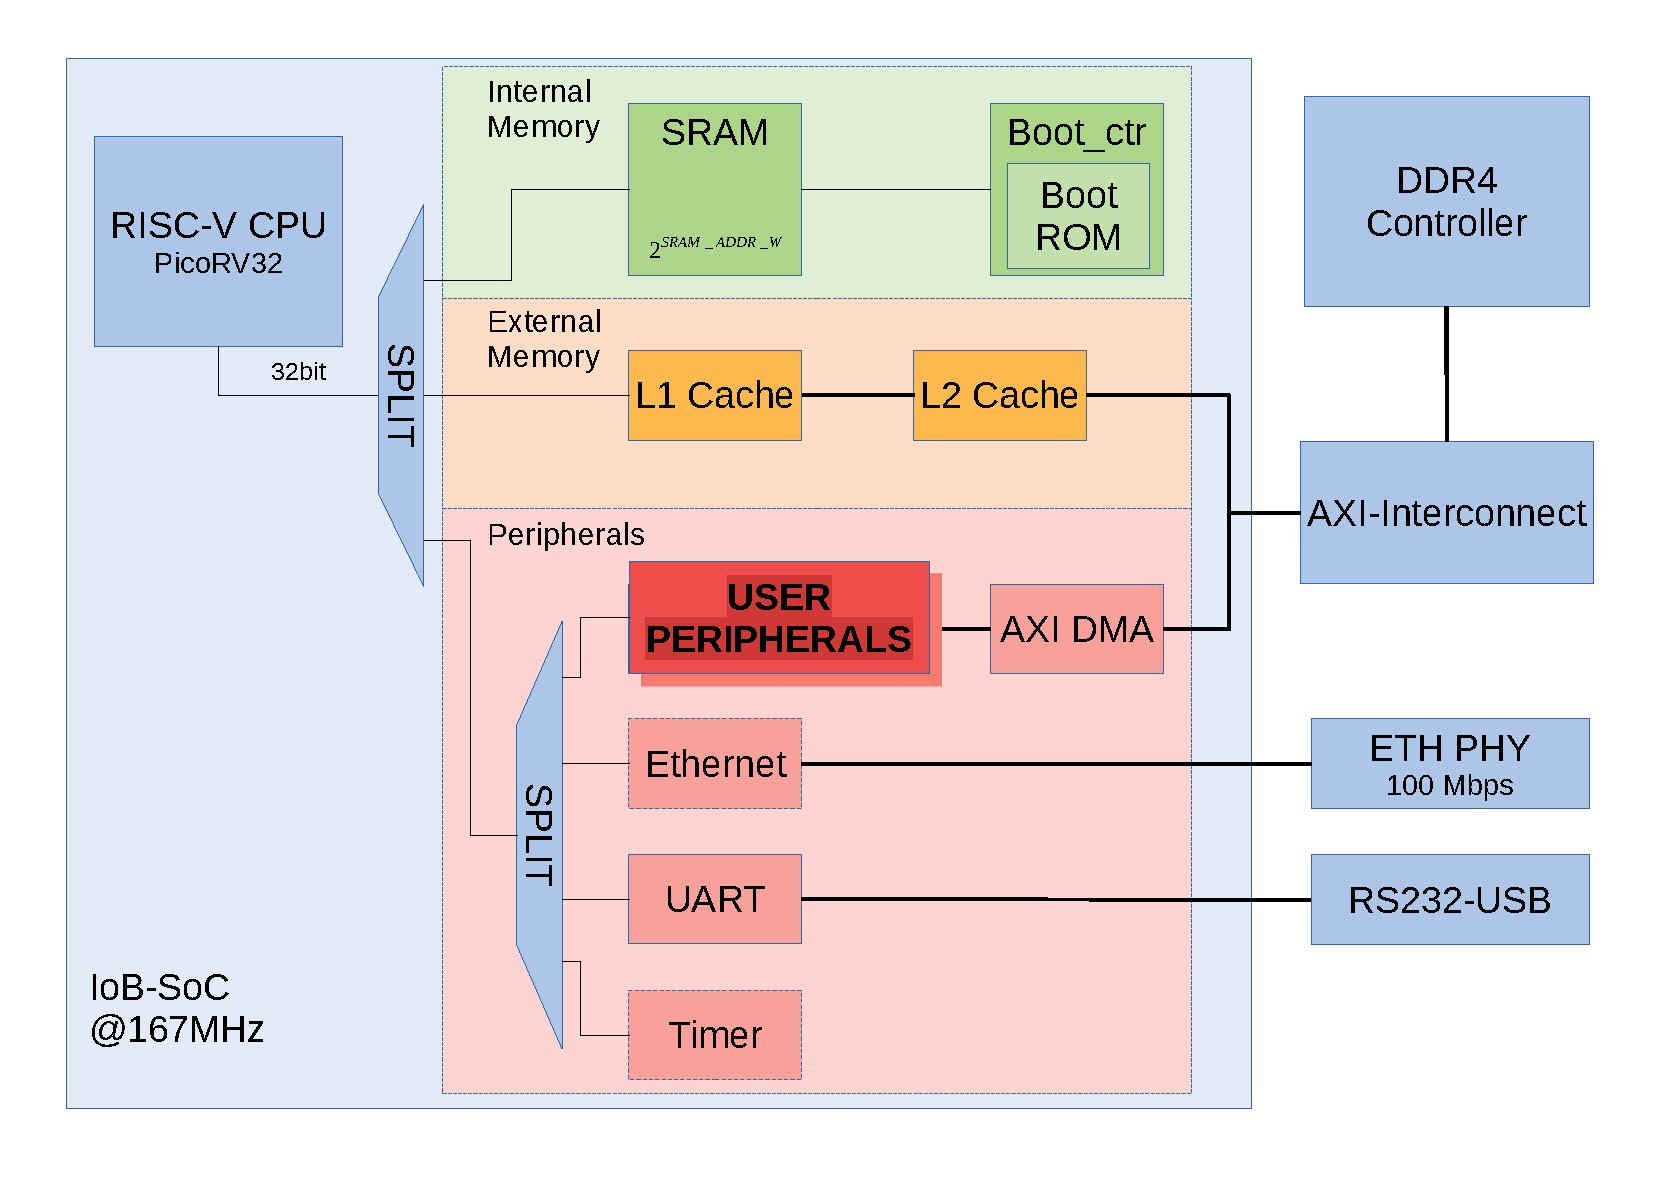
\includegraphics[width=\linewidth]{images/bd_original.pdf}
  \caption{\textit{IOb-SoC} sketch.}
  \label{fig:bd_original}
\end{figure}

Building a new processor-based system from scratch can take time and effort. The IObundle developers created the \textit{IOb-SoC} to facilitate this process. This work develops a variant of the existing \textit{IOb-SoC} capable of running a Linux Operating System. \textit{IOb-SoC} currently supports two FPGA board models: the Xilinx Kintex UltraScale KU040 Development Board and the Cyclone V GT FPGA Development Kit.


%%%%%%%%%%%%%%%%%%%%%%%%%%%%%%%%%%%%%%%%%%%%%%%%%%%%%%%%%%%%%%%%%%%%%%
\subsection{Sub-section...}

More text...
